%%\documentclass[a4paper,12pt,oneside]{llncs}
\documentclass[12pt,letterpaper]{article}
\usepackage[right=2cm,left=3cm,top=2cm,bottom=2cm,headsep=0cm]{geometry}

%%%%%%%%%%%%%%%%%%%%%%%%%%%%%%%%%%%%%%%%%%%%%%%%%%%%%%%%%%%
%% Juego de caracteres usado en el archivo fuente: UTF-8
\usepackage{ucs}
\usepackage[utf8x]{inputenc}

%%%%%%%%%%%%%%%%%%%%%%%%%%%%%%%%%%%%%%%%%%%%%%%%%%%%%%%%%%%
%% Juego de caracteres usado en la salida dvi
%% Otra posibilidad: \usepackage{t1enc}
\usepackage[T1]{fontenc}

%%%%%%%%%%%%%%%%%%%%%%%%%%%%%%%%%%%%%%%%%%%%%%%%%%%%%%%%%%%
%% Ajusta maergenes para a4
%\usepackage{a4wide}

%%%%%%%%%%%%%%%%%%%%%%%%%%%%%%%%%%%%%%%%%%%%%%%%%%%%%%%%%%%
%% Uso fuente postscript times, para que los ps y pdf queden y pequeños...
\usepackage{times}

%%%%%%%%%%%%%%%%%%%%%%%%%%%%%%%%%%%%%%%%%%%%%%%%%%%%%%%%%%%
%% Posibilidad de hipertexto (especialmente en pdf)
%\usepackage{hyperref}
\usepackage[bookmarks = true, colorlinks=true, linkcolor = black, citecolor = black, menucolor = black, urlcolor = black]{hyperref}

%%%%%%%%%%%%%%%%%%%%%%%%%%%%%%%%%%%%%%%%%%%%%%%%%%%%%%%%%%%
%% Graficos 
\usepackage{graphics,graphicx}

%%%%%%%%%%%%%%%%%%%%%%%%%%%%%%%%%%%%%%%%%%%%%%%%%%%%%%%%%%%
%% Ciertos caracteres "raros"...
\usepackage{latexsym}

%%%%%%%%%%%%%%%%%%%%%%%%%%%%%%%%%%%%%%%%%%%%%%%%%%%%%%%%%%%
%% Matematicas aun más fuertes (american math dociety)
\usepackage{amsmath}

%%%%%%%%%%%%%%%%%%%%%%%%%%%%%%%%%%%%%%%%%%%%%%%%%%%%%%%%%%%
\usepackage{multirow} % para las tablas
\usepackage[spanish,es-tabla]{babel}

%%%%%%%%%%%%%%%%%%%%%%%%%%%%%%%%%%%%%%%%%%%%%%%%%%%%%%%%%%%
%% Fuentes matematicas lo mas compatibles posibles con postscript (times)
%% (Esto no funciona para todos los simbolos pero reduce mucho el tamaño del
%% pdf si hay muchas matamaticas....
\usepackage{mathptm}

%%% VARIOS:
%\usepackage{slashbox}
\usepackage{verbatim}
\usepackage{array}
\usepackage{listings}
\usepackage{multirow}

%% MARCA DE AGUA
%% Este package de "draft copy" NO funciona con pdflatex
%%\usepackage{draftcopy}
%% Este package de "draft copy" SI funciona con pdflatex
%%%\usepackage{pdfdraftcopy}
%%%%%%%%%%%%%%%%%%%%%%%%%%%%%%%%%%%%%%%%%%%%%%%%%%%%%%%%%%%
%% Indenteacion en español...
\usepackage[spanish]{babel}

\usepackage{listingsutf8}
% Para escribir código en C
% \begin{lstlisting}[language=C]
% #include <stdio.h>
% int main(int argc, char* argv[]) {
% puts("Hola mundo!");
% }
% \end{lstlisting}


\title{Práctica 2}
\author{Jesús Rodríguez Heras\\
	Arantzazu Otal Alberro}

\begin{document}
	
	\maketitle
%	\begin{abstract} %Poner esto en todas las prácticas de PCTR
%%		\begin{center}
%%			\noindent
%			
%%		\end{center}
%	\end{abstract}
	\thispagestyle{empty}
	\newpage
	
%	\tableofcontents
%	\newpage
	
	%%\listoftables
	%%\newpage
	
	%%\listoffigures
	%%\newpage
	
	%%%% REAL WORK BEGINS HERE:
	
	%%Configuracion del paquete listings
	\lstset{language=bash, numbers=left, numberstyle=\tiny, numbersep=10pt, firstnumber=1, stepnumber=1, basicstyle=\small\ttfamily, tabsize=1, extendedchars=true, inputencoding=utf8/latin1, breaklines=true}
	
\section{Instalación de máquinas virtuales mediante Vagrant}
En esta primera parte vamos a crear el entorno de trabajo, consistente en tres máquinas virtuales pertenecientes a una misma red privada. Las máquinas se tendrán que crear a partir de un mismo fichero Vagrant.
\begin{enumerate}
	\item VM1, con IP 192.168.2.101
	\item VM2, con IP 192.168.2.102
	\item VM3, con IP 192.168.2.103
\end{enumerate}

Las máquinas tendrán la siguiente configuración:
\begin{itemize}
	\item nmap tiene que estar instalado en todos.
	\item iptables en la máquina VM1.
	\item ufw en la máquina VM1 (debería estar instalado por defecto).
	\item fwbuilder.
\end{itemize}

La instalación de los paquetes se deberá realizar mediante la provisión de Vagrant.

Para inicializar Vagrant usamos \texttt{vagrant init debian/jessie64} y luego abrimos y modificamos el archivo \texttt{Vagrantfile} de la siguiente forma:
\lstinputlisting[language=Ruby]{../Vagrantfile}

A continuación, iniciamos las tres máquinas virtuales en terminales diferentes con \texttt{vagrant up vmX} y nos conectamos a ellas mediante \texttt{vagrant shh vmX} (siendo ``X'' el número de la máquina virtual comprendido entre 1 y 3).

Para instalar nmap en todas las máquinas usaremos el aprovisionamiento de Vagrant creando el archivo \texttt{bootstrap.sh} siguiente:
\lstinputlisting[language=Bash]{../bootstrap.sh}

\section{Visibilidad de las máquinas}
Para los distintos ejercicios, se identifica a las máquinas como VM1, VM2 y VM3. Por comodidad, es recomendable poder usar nombres en las reglas. Para ello, se puede añadir en \texttt{/etc/hosts} una línea asociando un nombre y una IP con la siguiente sintáxis: IP NOMBRE ALIAS.

Para hacer esto, entramos en las tres máquinas virtuales y accedemos al archivo mencionado con \texttt{sudo nano /etc/hosts} y lo modificamos de la siguiente forma:
\begin{lstlisting}[language=Bash]
	192.168.2.101 vm1
	192.168.2.102 vm2
	192.168.2.103 vm3
\end{lstlisting}

\section{Configuraciones IPtables}
\subsection{Primeras pruebas}
En este ejercicio se pide testear VM1 desde VM2, realizando los siguientes ejercicios:
\begin{enumerate}
	\item \textbf{Desde VM2 comprobar los puertos que VM1 tiene abiertos.} \\
	Para comprobar los puertos usamos: \texttt{nmap vm1}.
	\item \textbf{Prohibir el acceso por ssh.} \\
	Para ello usaremos: \texttt{sudo iptables -A INPUT -p tcp ---dport 22 -j DROP}
	\item \textbf{Responde a las siguientes preguntas:}
	\begin{itemize}
		\item \textbf{¿Qué ha pasado?} \\
		La consola se queda bloqueada sin poder establecer conexión por ssh.
		\item \textbf{¿Puedo crear una nueva conexión?} \\
		Es imposible.
		\item \textbf{¿La consola sigue funcionando?} \\
		No, se queda bloqueada y no responde.
	\end{itemize}
\end{enumerate}

\subsection{Configuración mínima}
En los ejercicios siguientes, siempre debe partir de esta configuración:
\begin{itemize}
	\item \textbf{Permitir conexiones locales.} \\
	\texttt{sudo iptables -A INPUT -i lo -j ACCEPT}
	\item \textbf{Permitir conexiones ya establecidas.} \\
	\texttt{sudo iptables -A INPUT -m state ---state ESTABLISHED -j ACCEPT}
	\item \textbf{Políticas por defecto de rechazar en input.} \\
	\texttt{sudo iptables -A INPUT -j DROP}
\end{itemize}

Para comprobar estas configuraciones hicimos ping entre las máquinas para ver la conectividad.

\subsection{Configurando servidor web completo}
Configurar VM1 para que tenga la configuración de un servidor web, permitiendo:
\begin{itemize}
	\item \textbf{Todos se conecten a los puertos http y https.} \\
	Primero mostramos las iptables con \texttt{sudo iptables -L} y, si tenemos la anterior que no permitía conexiones entrantes, usamos \texttt{sudo iptables -F} para borrarlas todas\footnote{Si queremos borrar solo una regla, mostramos todas las reglas existentes con \texttt{sudo iptables -L --line-numbers} y para borrar la que queramos usamos \texttt{sudo iptables -D INPUT numeroderegla}} (con el inconveniente de que tendremos que reescribir las que queramos).\\
	Para habilitar http usamos: \texttt{sudo iptables -A INPUT -p tcp ---dport 80 -j ACCEPT} \\
	Para habilitar https usamos: \texttt{sudo iptables -A INPUT -p tcp ---dport 443 -j ACCEPT}
	\begin{figure}[h]
		\centering
		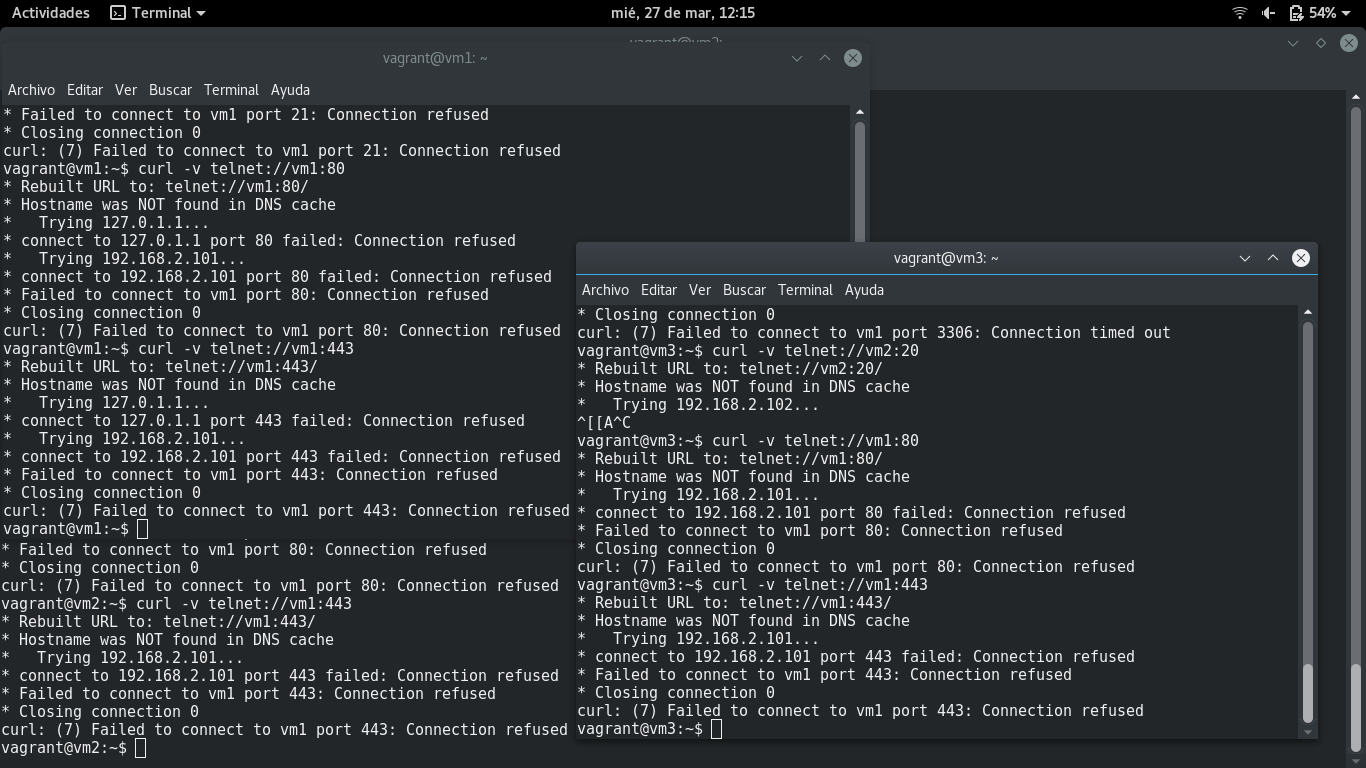
\includegraphics[scale=0.34]{http.png}
	\end{figure}
	\item \textbf{Conexión únicamente por parte de VM2 al servidor ftp.} \\
	\texttt{sudo iptables -A INPUT -p tcp ---dport 20 -s 192.168.2.102 -j ACCEPT}\\
	\texttt{sudo iptables -A INPUT -p tcp ---dport 21 -s 192.168.2.102 -j ACCEPT}
	\begin{figure}[h]
		\centering
		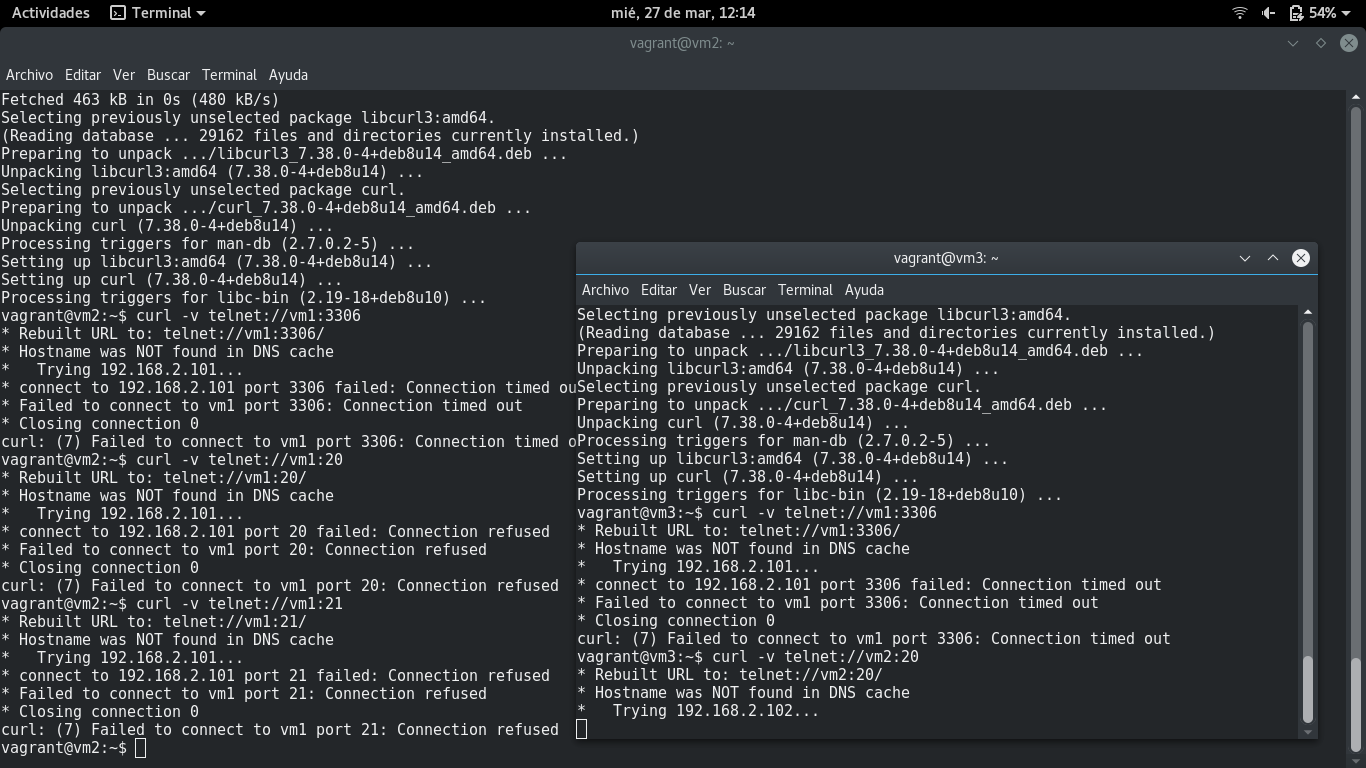
\includegraphics[scale=0.34]{ftp.png}
	\end{figure}
\newpage
	\item \textbf{Configurar VM1 para que sólo se pueda conectar localmente a mysql.} \\
	\texttt{sudo iptables -A INPUT -p tcp -i lo ---dport 3306 -j ACCEPT}
	\begin{figure}[h]
		\centering
		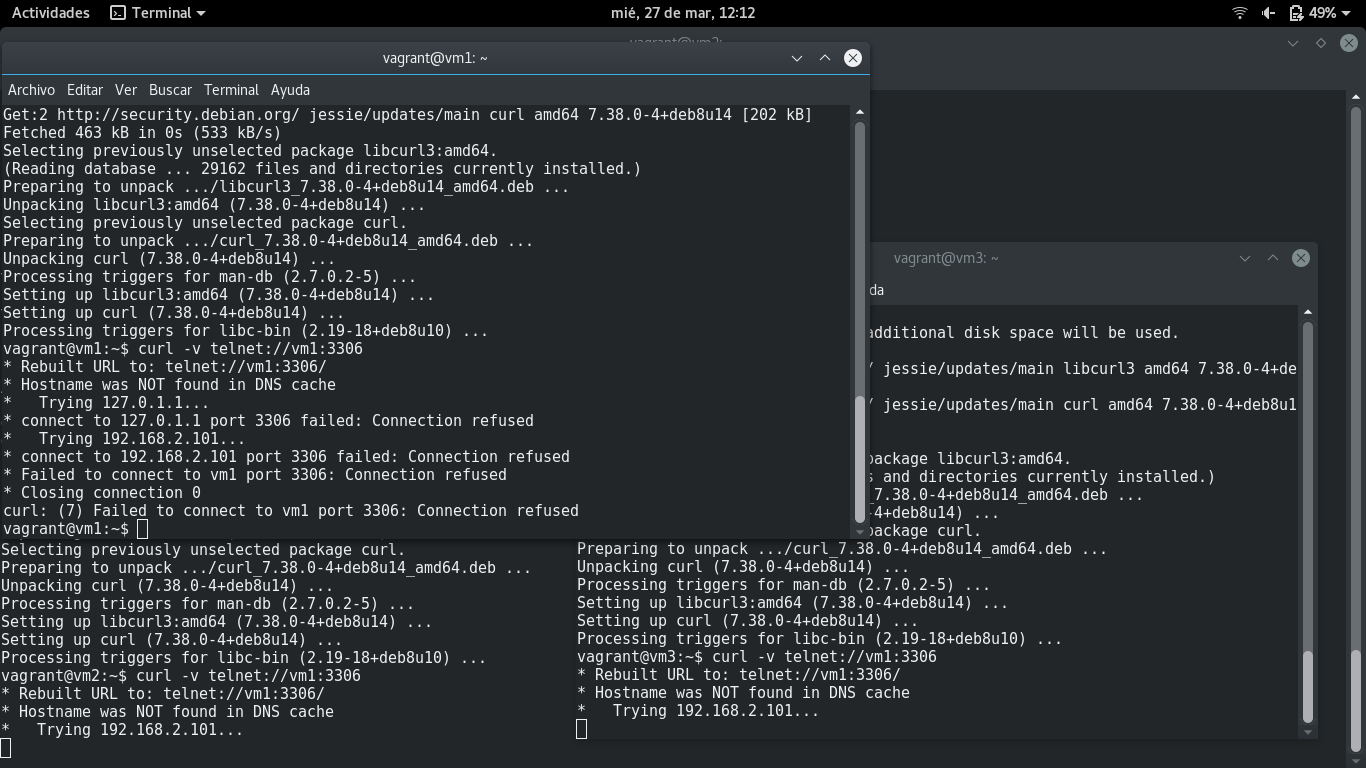
\includegraphics[scale=0.34]{mysql.png}
	\end{figure}
\end{itemize}

Otra opción para comprobar los puertos abiertos es poner el comando \texttt{nc -l numerodepuerto \&}. Eso nos abrirá e puerto que queramos y lo mandará a segundo plano con la finalidad de que el nmap o el telnet nos indique que ese puerto está abierto y a la escucha. Para cerrarlo, tendremos que poner el comando \texttt{kill -9 PID}, siendo PID el PID del proceso que nos mantiene el puerto abierto (que se nos muestra al mandar a segundo plano el comando \texttt{nc}).5

\newpage
\subsection{Poniendo excepciones}
Permitir conectar a VM1 desde VM2 y VM3 el acceso a los puertos desde 1:1000, con la excepción de que VM2 no se puede conectar por FTP.

Para VM2: \texttt{sudo iptables -A INPUT -p tcp ---dport 20:21 -s 192.168.2.102 -j DROP;sudo iptables -A INPUT -p tcp ---dport 1:1000 -s 192.168.2.101 -j ACCEPT}

Para VM3: \texttt{sudo iptables -A INPUT -p tcp ---dport 1:1000 -s 192.168.2.103 -j ACCEPT}

\begin{figure}[h]
	\centering
	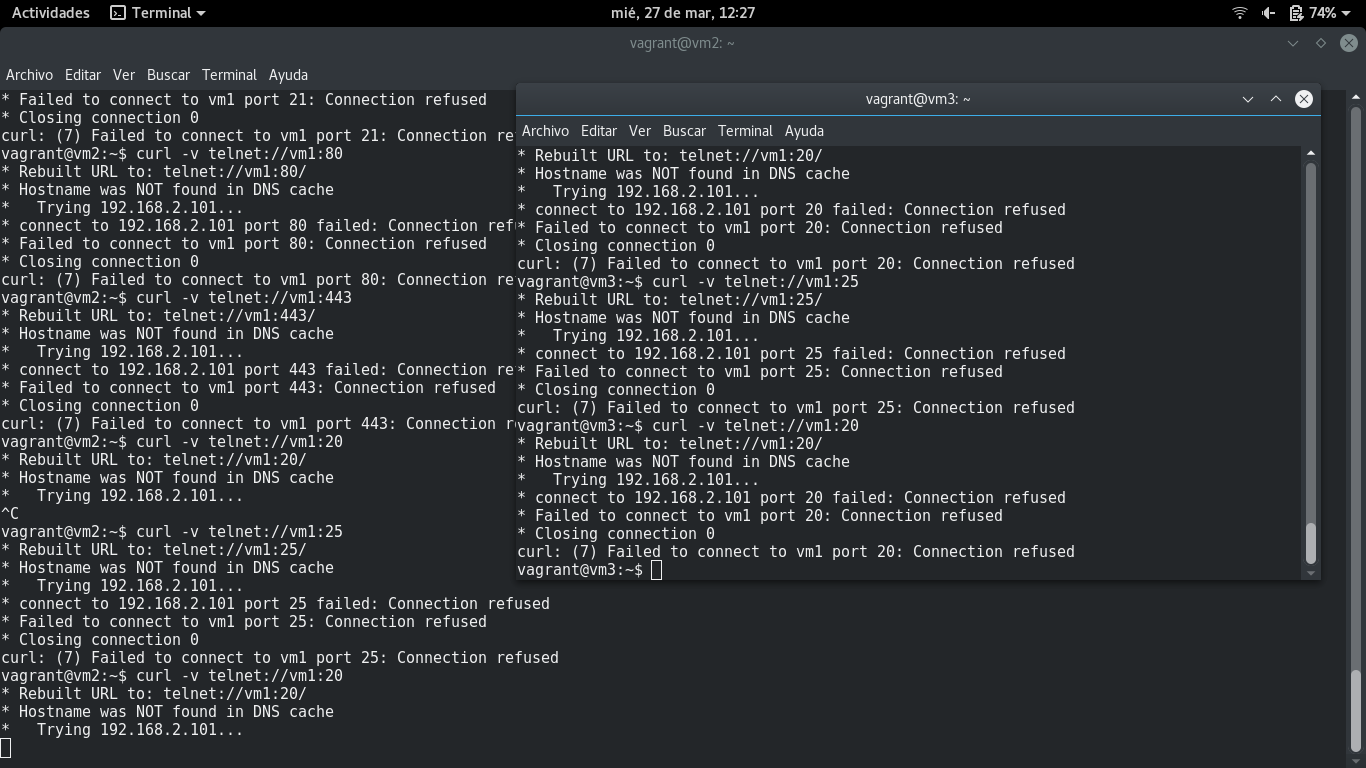
\includegraphics[scale=0.34]{1al1000.png}
\end{figure}

\newpage
\section{UFW}
Configurar VM1 para que tenga la configuración de un servidor web, permitiendo:
\begin{itemize}
	\item \textbf{Todos se conecten a los puertos http y https.} \\
	Para habilitar http usamos: \texttt{sudo ufw allow http} \\
	Para habilitar https usamos: \texttt{sudo ufw allow https}
	\begin{figure}[h]
		\centering
		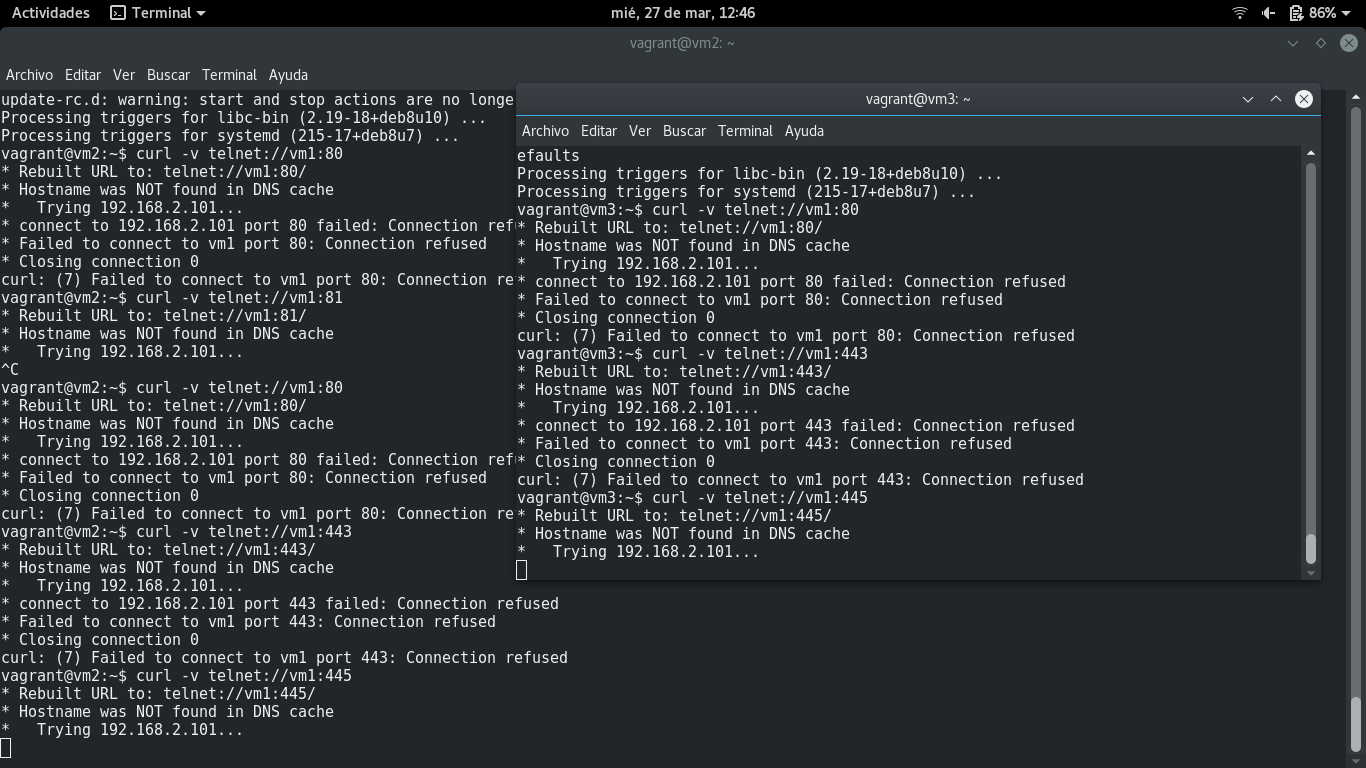
\includegraphics[scale=0.34]{http2.png}
	\end{figure}
\newpage
	\item \textbf{Conexión únicamente por parte de VM2 al servidor ftp.} \\
	\texttt{sudo ufw allow from 192.168.2.102 to any port 20}\\
	\texttt{sudo ufw allow from 192.168.2.102 to any port 21}
	\begin{figure}[h]
		\centering
		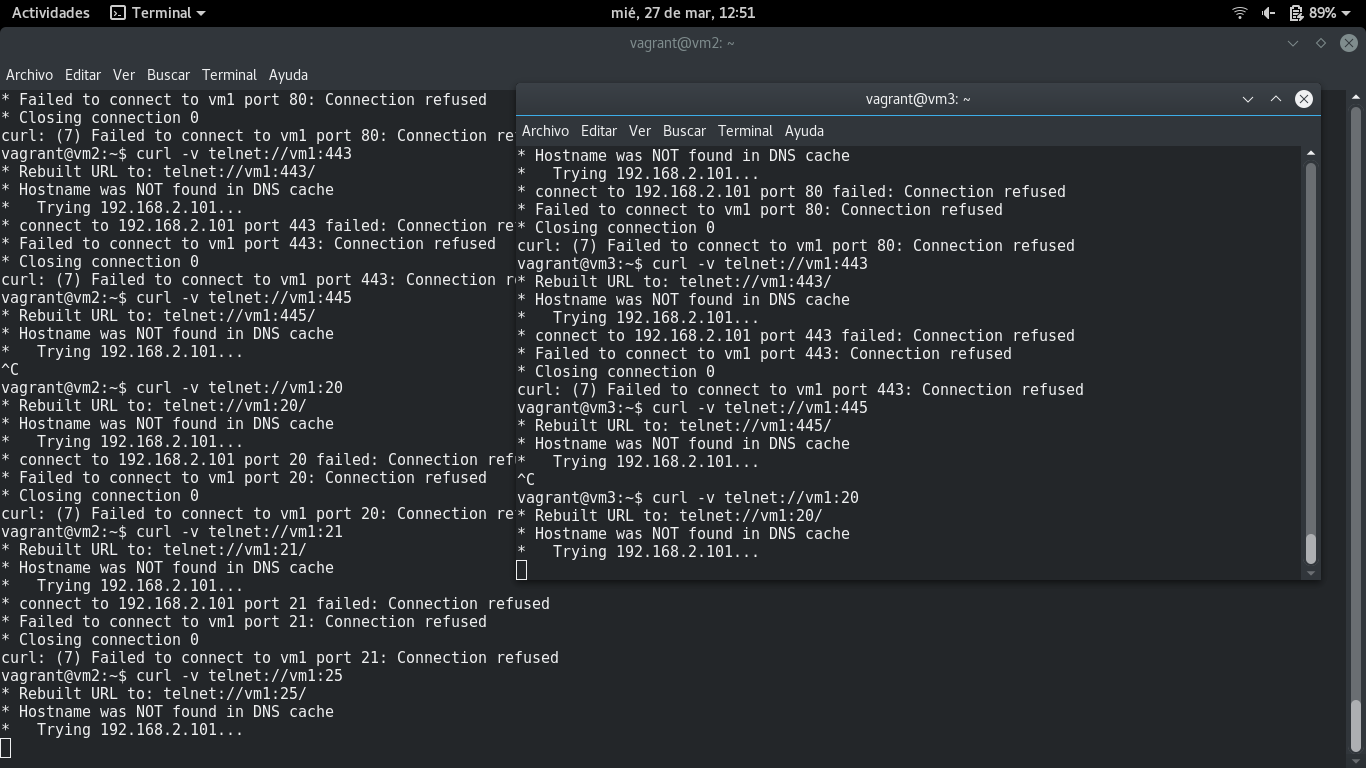
\includegraphics[scale=0.34]{ftp2.png}
	\end{figure}
	\newpage
	\item \textbf{Configurar VM1 para que sólo se pueda conectar localmente a mysql.} \\
	\texttt{sudo ufw allow from 192.168.2.101 to any port 3306}
	\begin{figure}[h]
		\centering
		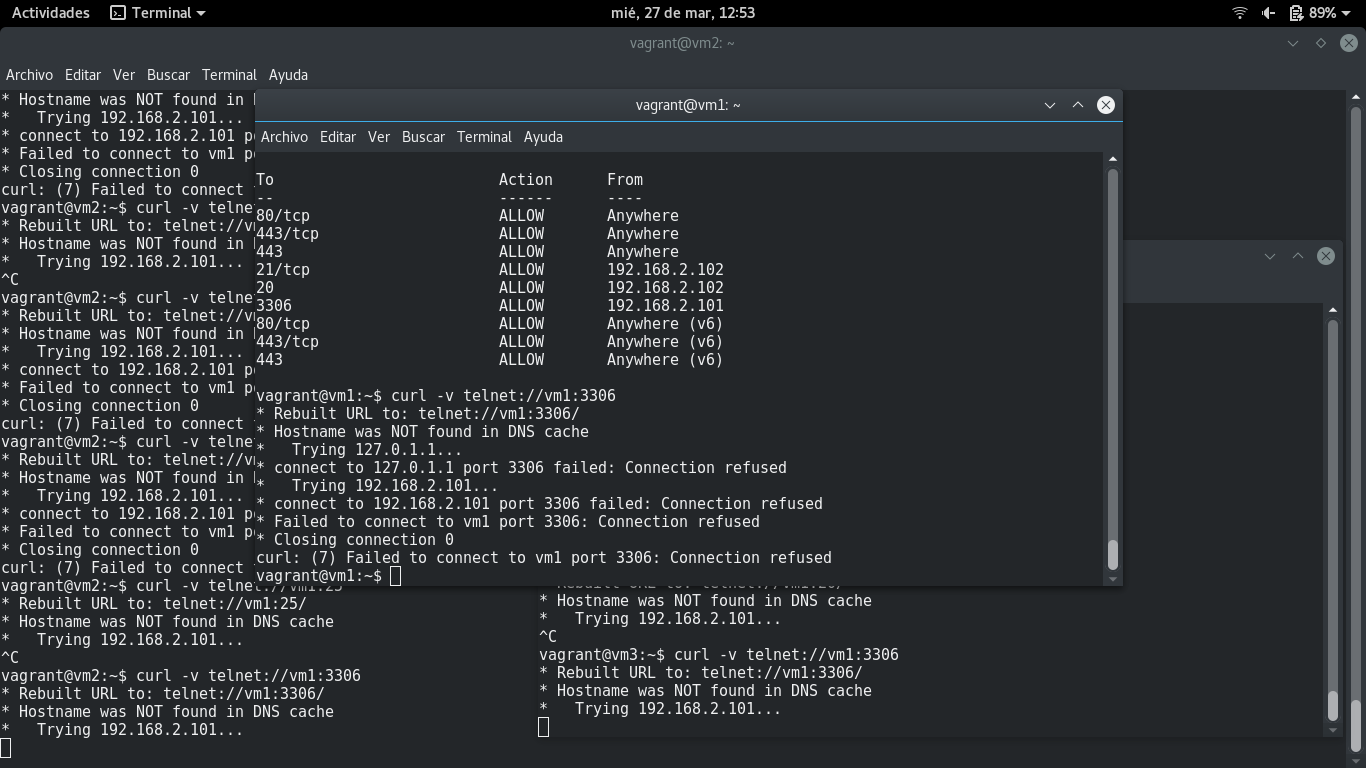
\includegraphics[scale=0.34]{mysql2.png}
	\end{figure}
\end{itemize}

\end{document}